\documentclass{report}
\usepackage[parfill]{parskip}
\usepackage{todonotes}
\usepackage{hyperref}
\usepackage{amsmath}
\usepackage{wrapfig}
\usepackage{graphicx}
\usepackage{textcomp}
\usepackage{bytefield}
\graphicspath{ {./img/} }
\begin{document}

\title{NEA: Font Rasterizer}
\author{Jake Irvine}

\maketitle
\chapter{Analysis}

Text is a key aspect of how we interact with machines. Virtually everything that
is done on a computer requires some form of reading on a screen. The program
that converts the binary text data to pixels on a screen is a `font engine' or
`font rasterizer'. These take some text or a single character and output a
texture which will get copied into the screen buffer. There is another component
of font rendering, which arranges individual characters output by a font
rasterizer into words or paragraphs, called a layout engine.

Creating a full font engine is a very large task - the TrueType format (the
industry standard for font files) is a very large specification, and can be
further enhanced by vendor-specific extensions. For example, some fonts contain
small programs inside them that adjust the actual glyphs to better fit the pixel
grid of the screen. These are implemented in a custom virtual machine that is
very complex and time consuming to create. However, when rendering characters at
a large scale, the impact of these features is far less, yet still comes at a
substancial performance cost.

My project has two parts: the parser and the renderer itself. The parser will
take a TrueType font file and output the bezier curves of the selected
character, by reading the binary file. This is non-trivial, because the TrueType
format is relatively complex, and contains a lot of optional features (which
this project will largely ignore, unless I have time left over). I will
investigate parser-combinator systems and either use that or create my own
custom parser architecture.

TrueType fonts are composed of straight line segments and bezier curves. These
are primitives that are relatively easy to draw to the screen quickly, and are
what the rendering portion of my project will involve. I will initially render
at a high resolution, to avoid the need for anti-aliasing and reduce the
possibility of artifacts (pixels out of place, etc) in the process. I will
potentially implement some form of anti-aliasing at some point, depending on how
well the rest of the project goes.

\section{Project Scope}
The TrueType format is very complex, and creating a full implementation is
outside the scope of a NEA. For simplicity, I will focus on the most important
part of the format: individual character glyphs. This avoids the need for
parsing kerning data, ligatures, and other optional features that would be
present in a full implementation. In addition, I will not implement the
grid-fitting aspect of the specification, as this would require creating a
virtual machine to run the instructions contained in the font.

\todo{add to this later as i find more stuff i can't do}


\section{Existing Solutions}
\subsection{SDL\_ttf}
SDL\_ttf is a ready to use library for rendering fonts to a texture using the
SDL graphics library. Internally, it uses the freetype library, which is
discussed below.

Advantages:
\begin{itemize}
\item{Simple to integrate into applications.}
\item{Uses the freetype backend, which supports a wide range of font features.}
\item{Can be compiled for any platform, due to the fact that it's written
    using crossplatform libraries and C++.}    
\end{itemize}

Disadvantages:
\begin{itemize}
\item{Slower than using freetype alone, because it adds SDL bindings on top of
    it.}
\item{Can only render on the CPU, failing to take advantage of any GPU that may
    be present.}
\item{Since it uses SDL for rendering, it can be quite hard to use with a non
    SDL project.}
\item{Due to it's simple API, it fails to expose many advanced features of
    freetype, that might be useful to a client.}
\end{itemize}

\subsection{freetype}
Freetype is a free, open source font engine that is used in many large software
projects, such as GNU/Linux, iOS and Postscript. It supports the vast majority
of font features and formats, including little-used ones such as .FON files and
X11 PCF fonts. However, due to this, it is very large, and rather slow.

Advantages:
\begin{itemize}
\item{Can handle virtually any font format you may need.}
\item{A full implementation of the TrueType specification, meaning it supports
    all of the features of the specification, as well as a number of vendor
    specific extensions.}
\item{Will run on a wide variety of systems, including the 16-bit Atari and
    Amiga computers.}
\item{Supports a wide range of character encodings, including the full unicode
    range of encodings, such as UTF-8 and UTF-16.}
\end{itemize}

Disadvantages:
\begin{itemize}
\item{Slow, due to it's support of the full specification.}
\item{Has a large memory footprint, meaning there is less space available for
    other programs.}
\item{Has a relatively complex API, that can be harder to integrate into
    applications already using a different font engine.}
\item{It does not handle complex layouts, which may be useful for some users.}
\end{itemize}

\subsection{Quartz}
Quartz is the font renderer used on MacOS and iOS devices, for almost all
software. It uses subpixel positioning, which means each glyph doesn't have to
be aligned with the pixel grid, instead being allowed to be anywhere between
pixels, using subpixel rendering and anti-aliasing to properly handle this
case.

Whilst this can result in clearer display at high dpi resolutions, (such as
Apple's retina displays), at lower dpi monitors or smaller font sizes it can
result in harder to read text.

Advantages:
\begin{itemize}
  \item{Provides the closest similarity to printed text when viewed on high DPI
      displays. }
  \item{Is included by default with MacOS and iOS}
\end{itemize}

Disadvantages:
\begin{itemize}
\item{Will only run on MacOS / iOS devices}
\item{The subpixel grid can make fonts look blurry at low DPI monitors.}
\end{itemize}
\newpage
\section{Project Background}

\subsection{Domain Terminology}
\textbf{Font Family}: a collection of typefaces, at different weights, or styles
such as italics.
\\
\textbf{Typeface}: commonly referred to as a font, a typeface is a style of
lettering that can be displayed on the screen or in print.
\\
\textbf{Font}: an instance of a typeface at a specfic size.
\\
\textbf{Glyph}: the shape corresponding to a specific character in a specific font. 
\subsection{Bezier Curves}
Individual glyphs of a font are built up using \textit{outlines}, which are
themselves built of several segments of line and curve. More specifically, an
outline consists of a set of line segments and quadratic bezier curves, which
create a closed loop that forms all or part of the glyph. Luckily, both line
segments and bezier curves are fairly easy for computers to render, and have
been used in computer graphics since it's inception.

A quadratic bezier curve is described by the equation
\begin{equation*}
\mathbf{B}(t) = (1 - t)^2\mathbf{P}_0 +2(1 - t)t\mathbf{P}_1 + t^2\mathbf{P}_2
\end{equation*}
where $\mathbf{P}_0$, $\mathbf{P}_1$, $\mathbf{P}_2$ are the position vectors of
the 3 control points for the curve, as $t$ ranges from $0$ to $1$. We can draw
this in a similar way to how we draw line segments: for a sufficient sample rate
over $t$, we can evaluate $\mathbf{B}(t)$ and, rounding to the nearest pixel,
plot that point.

Similarly, we can describe a line segment (which is effectively a linear bezier
curve) using the following equation:
\begin{equation*}
  \mathbf{B}(t) = \mathbf{P}_0 + t(\mathbf{P}_1 - \mathbf{P}_0)
\end{equation*}
where $\mathbf{P}_0$, $\mathbf{P}_1$ are the two control points, the beginning
and end of the line segment. \todo{needs pictures}

\subsection{The Font Pipeline}

There are several stages involved in getting text to display on the screen.
First, the file containing the font is read. Often these are in a standard
folder, but all font systems support reading from arbutrary files. The file is
parsed (which means broken down into the data that's needed for the specific
task) and various tables in the font file are read. The glyph coordinate data
will then be parsed and read, usually into a cache.

Next is the hinting step. Because fonts are usually distributed as vectors, yet
they are being displayed on a fine pixel grid, naievely rendering them can
result in poor font quality. Hinting is an process of distorting the glyph to
better fit the pixel grid and size that it will be displayed on. A properly
hinted font contains a small program for each glyph, to be executced in a
virtual machine, that distorts the vector data to align with the pixel grid.
This is a very complex process that is responsible for most of the time
rendering the font.
\begin{wrapfigure}{r}{0.4\textwidth}
  \centering
  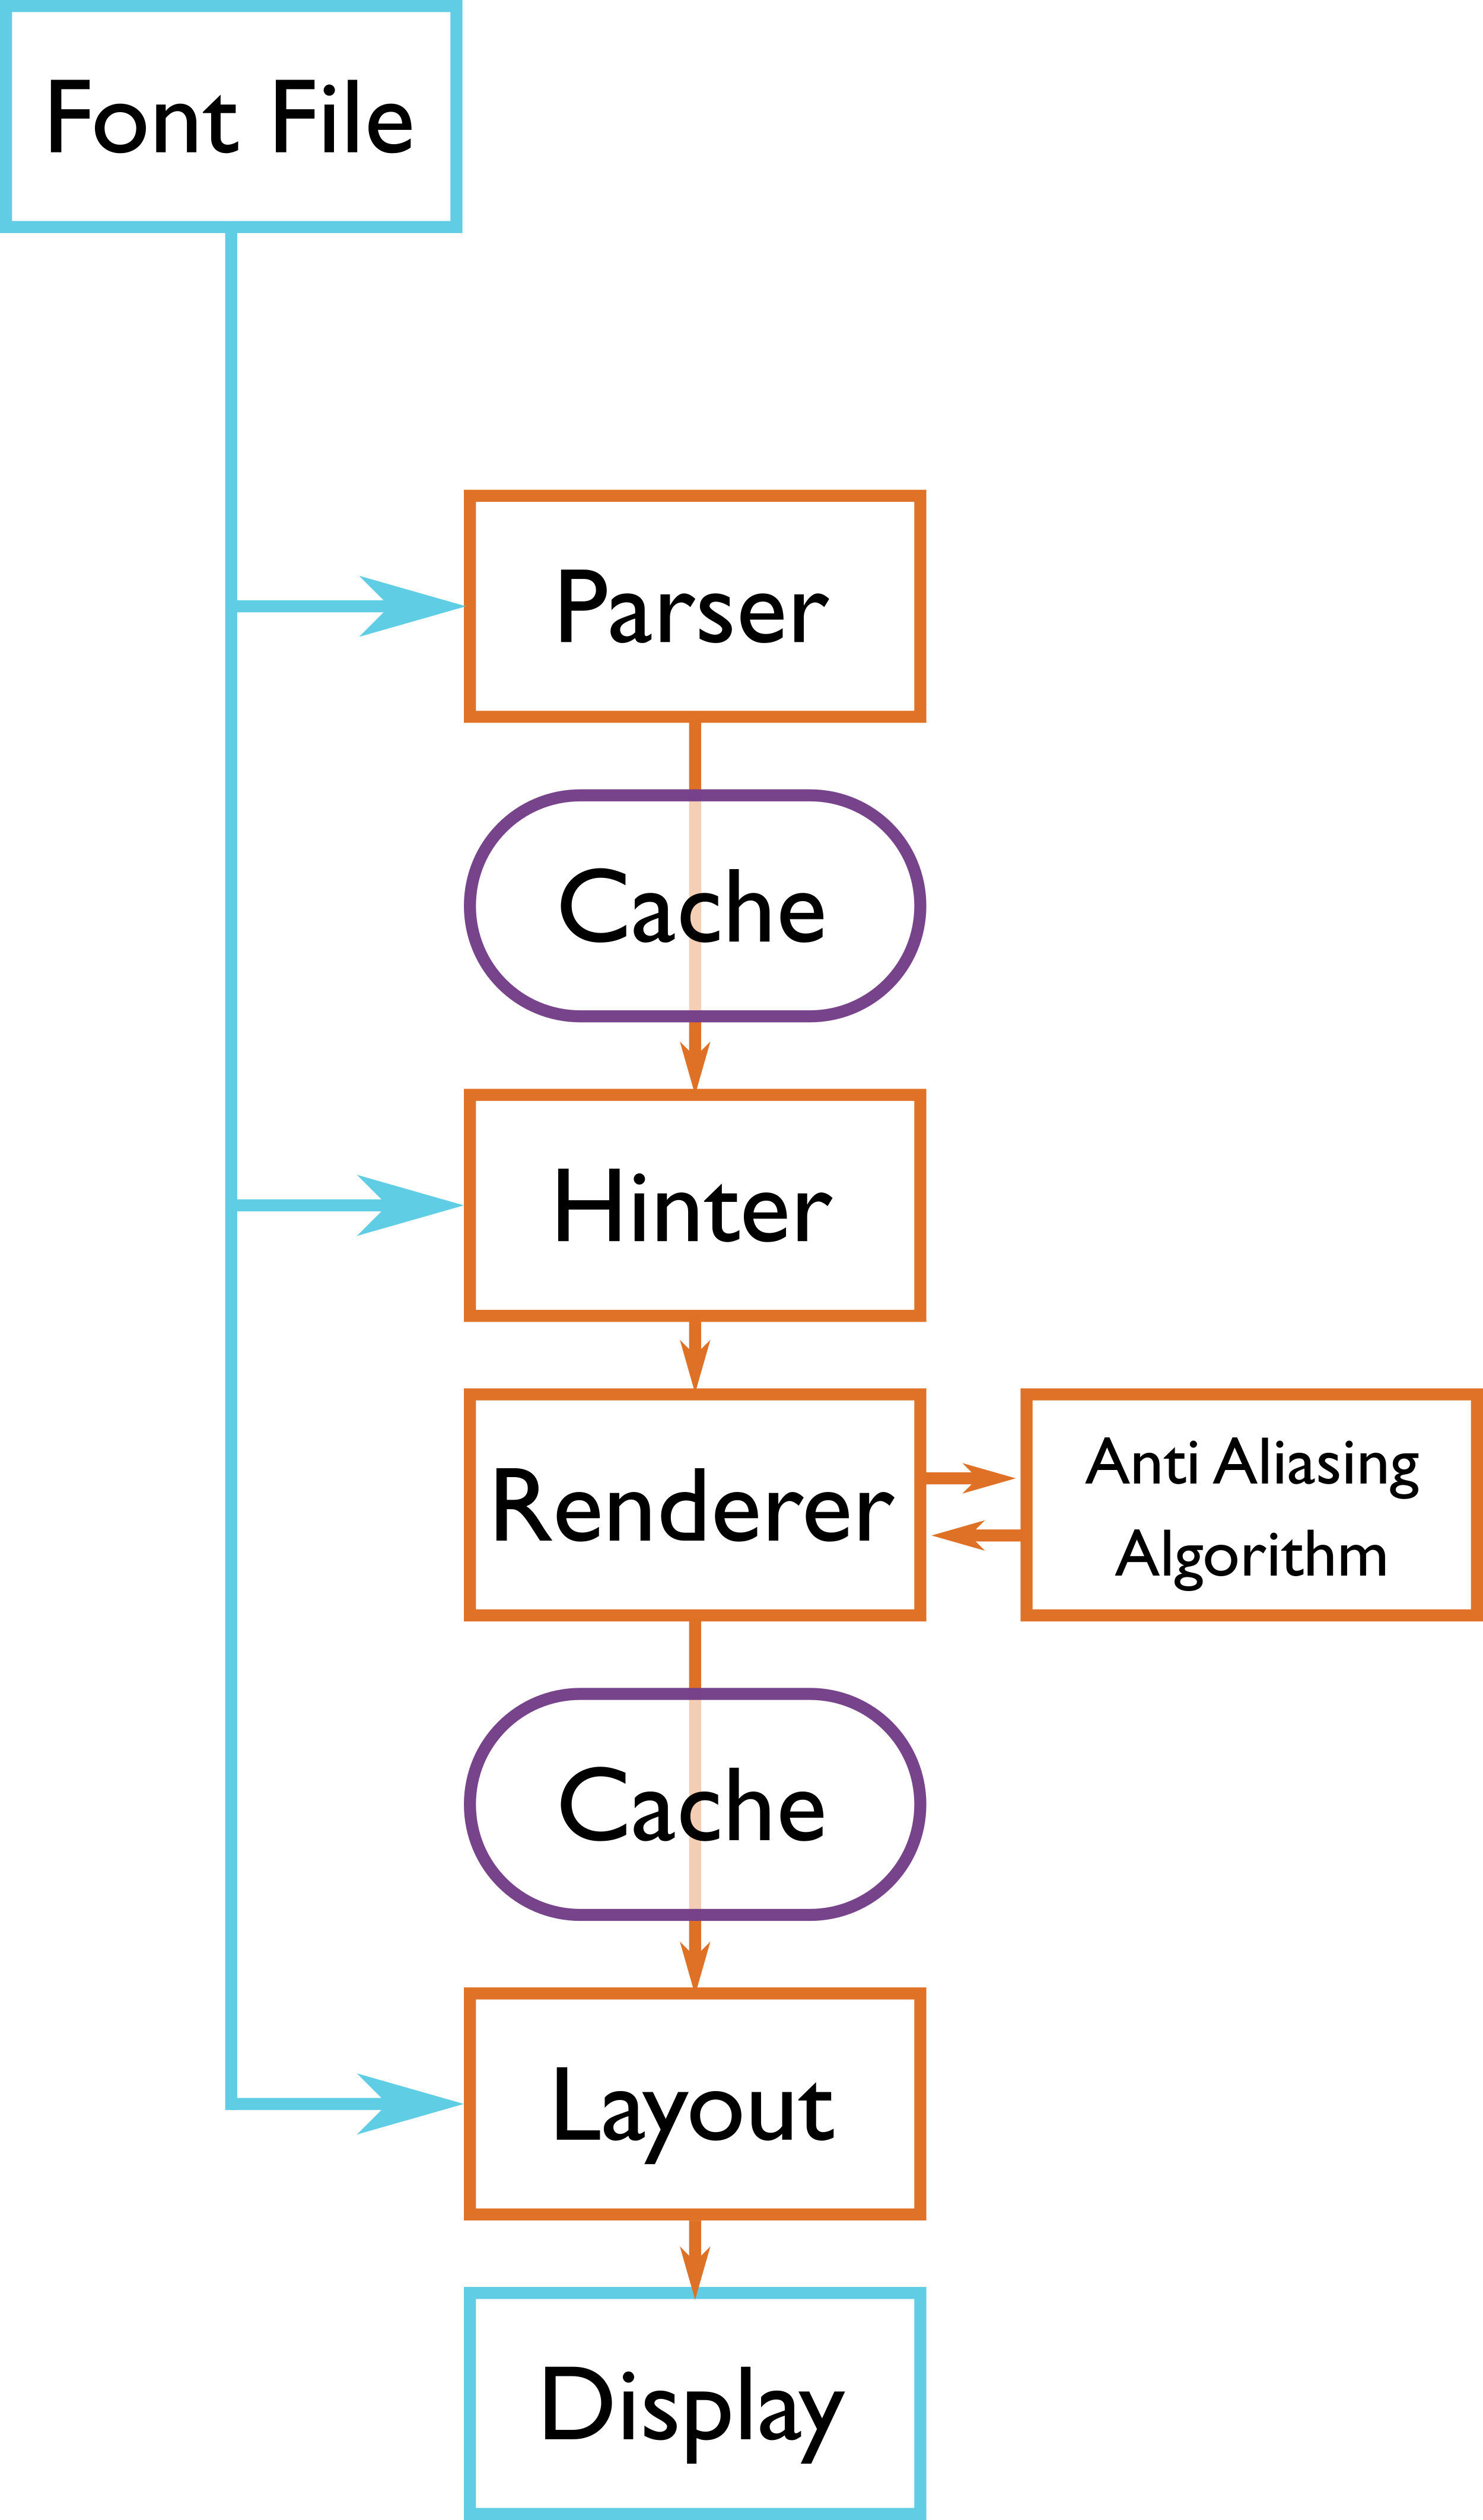
\includegraphics[width=0.4\textwidth]{fontpipelineimg}
\end{wrapfigure}

The hinted font is then rendered, taking the bezier curves of the font and
creating a raster image. This image is then anti-aliased, probably through
supersampling \todo{explain this more}, which is a process that turns a
black-and-white image to a greyscale one which looks sharper on the screen. Some
advanced anti-aliasing techniques take advantage of the RGB format of our
displays, to get a larger effective resolution to work with.

Finally, the anti-aliased image is displayed on the screen. The exact process
behind where it should be placed is handled by a layout engine, which is
responsible for forming individual glyphs into words and pages. A layout engine
still needs to reference the original font file, as kerning information which
dictates the individual spacing between characters is stored in a table there.

font file \rightarrow parser \rightarrow cache \rightarrow hinting \rightarrow
rendering \rightarrow anti-aliasing \rightarrow layout


\subsection{The TrueType Format}
A TrueType font file is a binary file that contains all the data needed to
display a font on the screen. The format, initially codenamed `Bass', was
designed by Apple in the 1980s for Mac System 7, and has continued to evolve and
is now used by virtually every consumer operating system and font engine. The
full specification is available at
\url{https://developer.apple.com/fonts/TrueType-Reference-Manual/}, which will
be summarized here.

A TrueType font is identified by the magic bytes (the first few bytes of many
file formats are different to aid in distinguishing them) \texttt{0x00010000}.
This is followed by a table directory which provides offsets to the various
tables used in the file. Each table contains some information about how the font
should be rendered, or metadata such as the font licence or author. For example,
the \texttt{kern} table contains data related to font kerning, which controls
the spacing between individual letters.

Of primary relevance to this project is the \texttt{glyf} table, which contains
the actual glyph data used in the character to be rendered. It is structured as
an array of glyphs, with each glyph as follows:

\begin{bytefield}[bitwidth=2.2em]{16}
  \bitheader{0-15} \\
  \begin{rightwordgroup}{Glyph header}
    \wordbox{1}{numberOfContours} \\
    \bitbox{16}{xMin} \\
    \bitbox{16}{xMax} \\
    \bitbox{16}{yMin} \\
    \bitbox{16}{yMax} 
  \end{rightwordgroup} \\

  \wordbox{3}{Either a simple glyph data structure, or a complex glyph data
    structure, dependent on the value of \texttt{numberOfContours}.}
\end{bytefield}
\\

\begin{bytefield}[bitwidth=2.2em]{16}
  \bitbox{16}{\textbf{Simple Glyph Data}} \\
  \bitheader{0-15} \\
  \wordbox{2}{Array of glyph contour endpoints, one word wide,
    \texttt{numberOfContours} long.} \\
  \wordbox{1}{instructionLength} \\
  \bitbox{8}{Instruction 1} & \bitbox{8}{Instruction 2} \\
  \bitbox{8}{Instruction 3} & \bitbox{8}{...} \\
  \bitbox{8}{...} & \bitbox{8}{Instruction $n$} \\
  \wordbox[tlr]{3}{Array of flags, length can be determined from the final
    endpoint index} \\
  \bitbox[l]{8} {Example:} & \bitbox{1}{C} & \bitbox{1}{xSh} & \bitbox{1}{ySh} &
  \bitbox{1}{R} & \bitbox{1}{xR} & \bitbox{1}{yR} & \bitbox{2}{Reserved} \\
  \wordbox[blr]{1}{}\\
  \wordbox{2}{Array of deltaX}\\
  \wordbox{2}{Array of deltaY}\\
  \\
  \\
  \bitbox{16}{\textbf{Complex Glyph Data}}\\
  \bitheader{0-15} \\
  \wordbox{1}{Flags (see full spec for details)}\\
  \wordbox{1}{Glyph Index}\\
  \wordbox{2}{\textit{variable size}\\Argument 1 (flag dependent)}\\
  \wordbox{2}{\textit{variable size}\\Argument 2 (flag dependent)}
\end{bytefield}

\textit{Note: Most uses of complex glyph tables are outside of the scope of this project.}
\\
\\
Using this table, and the \texttt{whatever the char map table is called}, we can
turn a single character into a set of curves and line segments that can be
scaled and drawn to the screen.

\section{Measurable Objectives}
\begin{enumerate}
  \item{The program will parse TTF files correctly, extracting character and
      glyph data from them.}
  \item{The program will display single characters on the screen in a specified
      font.}
  \item{The program will display these characters in a reasonable amount of
      time, say, not longer than a second (1000ms)}
  \item{The program will anti-alias these characters for improved readability}
  \item{The program will reject incorrectly formed TTF files in a safe manner}
\end{enumerate}

\chapter{Design}
\section{High Level Design}

\begin{wrapfigure}{r}{0.5\textwidth}
  \centering
  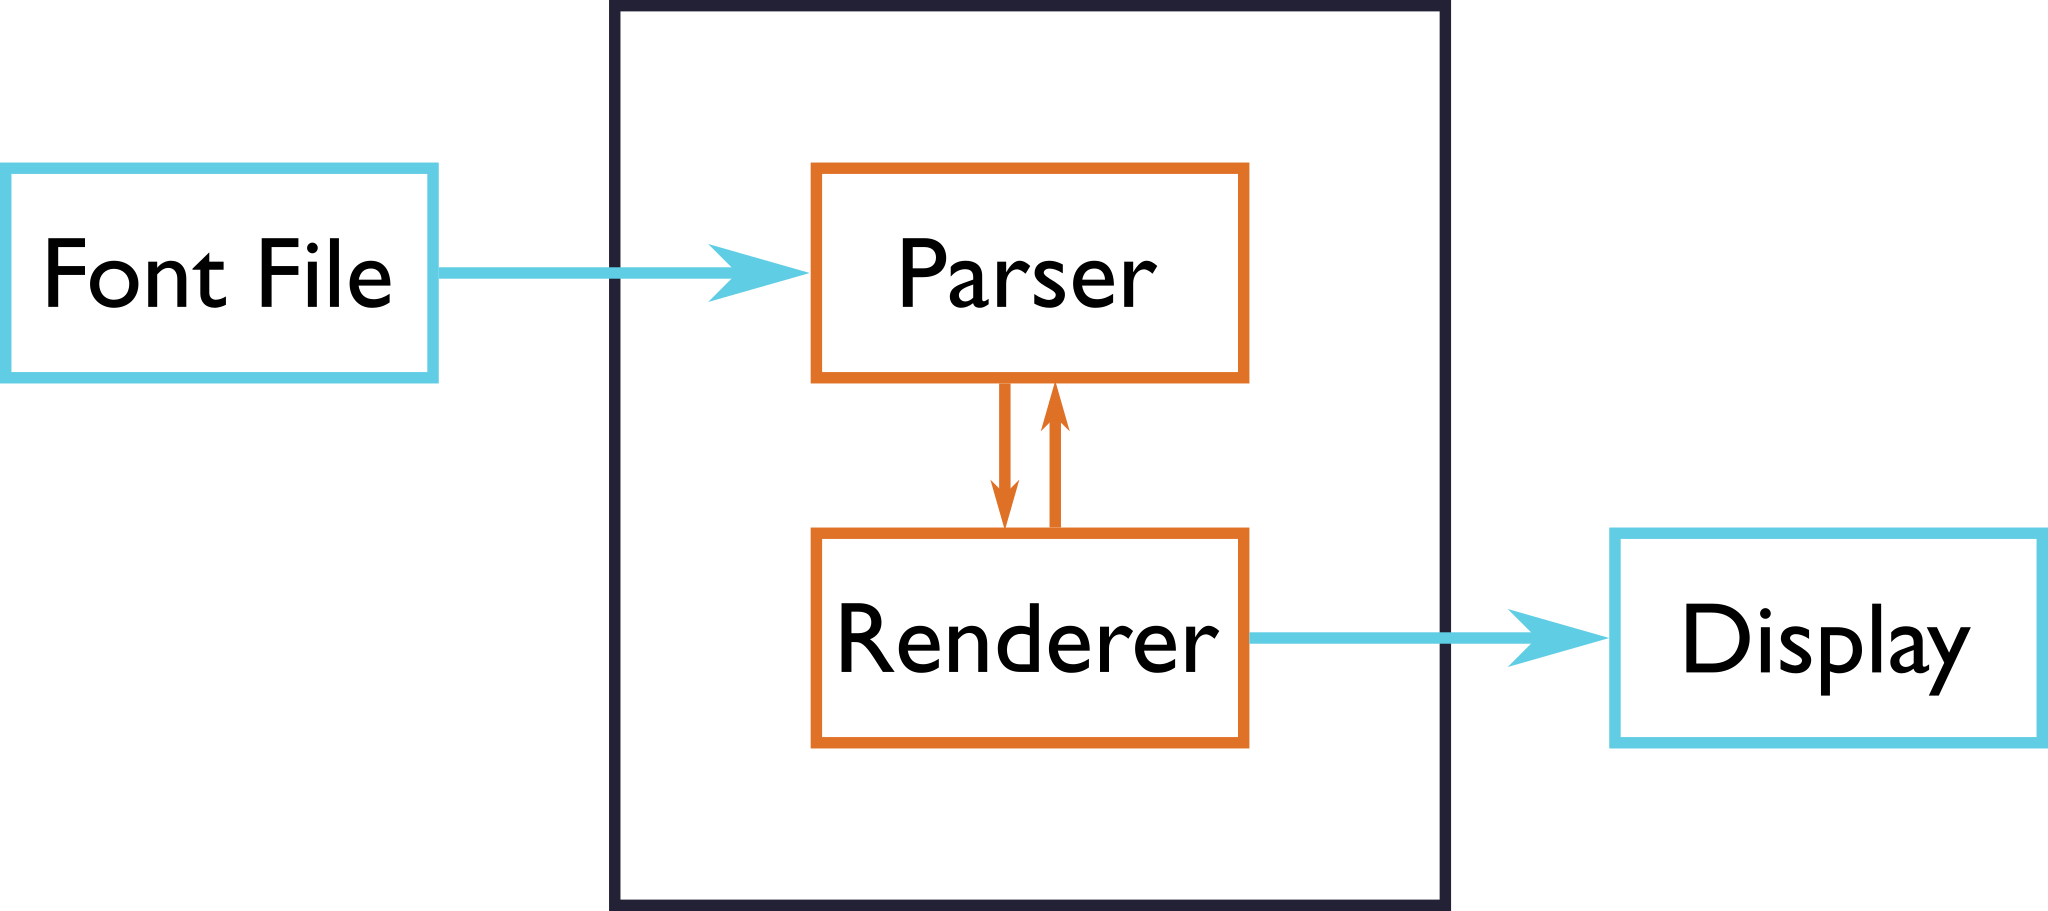
\includegraphics[width=0.5\textwidth]{design/highlevelout}
\end{wrapfigure}

The task has 2 clear subdivisions:
\begin{enumerate}
\item{Parsing the specified font file.}
\item{Displaying the parsed bezier curves on the screen.}
\end{enumerate}


I anticipate task 1 being the hardest, because the TrueType format is very
complex and requires sophisticated parsing to extract the data needed. In
contrast, rendering bezier curves to the screen is a task is moderately simple,
as the bezier curve is used frequently in computer graphics applications.

I will program in C++, using the cmake build system, and use the SDL graphics
library to display the GUI and rendered characters on the screen. Other
libraries involved will be \texttt{sdl\_ttf} for rendering the GUI text, and
\todo{perhaps} \texttt{sdl\_gfx} to simplify bezier curve rendering.

Whilst it may seem strange to include a different font rasterizer in a project
involving font rasterization, this rasterizer will be used only for the GUI, not
the actual display of characters itself. This is because, when debugging, the
GUI will need to remain in a functional state despite the font rasterizer itself
not being functional. Should the rasterizer get to a sufficiently stable state I
shall consider removing \texttt{sdl\_ttf} in favor of my own rasterizer.

\subsection{The Parser}
The parser needs to take the filename of a font, and by examining the associated
file, read various data about the font. The following is a loose list of the
data needed; other data may be needed to properly parse this, or for other
purposes.

\begin{enumerate}
  \item{The \texttt{head} table, which contains information about the rest of
      the file}
  \item{The \texttt{cmap} table, which contains the mapping between character
      and glyph index}
  \item{The \texttt{loca} table, which maps glyph indices to offsets from the
      start of the \texttt{glyf} table}
  \item{The individual glyph data, which requires the above data points to
      find in the file}
  \item{Various font metrics, contained in various tables around the font file}
\end{enumerate}

At the very beginning of the file is the table directory, which contains the
locations and length of all the font tables. Parsing this allows us to look up
the locations of the rest of the data in the file. Next we will examine the
\texttt{head} table to store important metrics that will be used elsewhere in
the file.

At this point, the program will prompt the user for the character that they
would like displayed. This character will be looked up in the \texttt{cmap}
table, to get a glyph index, and then the \texttt{loca} table, to convert the
index into a glyph offset and length.

Finally, we lookup the glyph in the \texttt{glyf} table, and store the entire
glyph data structure. This is quite complex to parse, and will have it's own
section of the program specifically. Parsing this will result in a list of
bezier curves to be rendered, which is then passed to the renderer.

\subsubsection{The \texttt{Font} class}
A key data structure in this project will be the \texttt{Font} class. This is a
large structure that contains, through composition, all the data needed to
display the font.

\begin{center}
  \begin{tabular}{|l|c|c|}
    \hline
    \multicolumn{3}{|c|}{The \texttt{Font} class} \\
    \hline
    \textbf{Type} & \textbf{Name} & \textbf{Access} \\
    \hline
    \texttt{std::map<std::string, TableData>} & tables & private \\
    \hline
    \texttt{std::map<char, Glyph>} & glyphs & private \\
    \hline
    \texttt{std::string} & fontName & private \\
    \hline
    \hline
    \textbf{Signature} & \textbf{Returns} & \textbf{Access} \\
    \hline
    \texttt{Font()} & Font & public \\
    \hline
    \texttt{parse(std::string filename)} & void & public \\
    \hline
    \texttt{glyphExists(char glyph)} & bool & public \\
    \hline
    \texttt{getGlyph(char glyph)} & Glyph* & public \\
    \hline
    \multicolumn{3}{|c|}{Plus many more private methods used for parsing...} \\
    \hline
  \end{tabular}
\end{center}

\subsubsection{The table directory}
This is at the beginning of the file; no offset is needed to find it. The first
few bytes are magic numbers and version information that will be checked, to
ensure that the file is in fact a TTF file. First, we check the initial 32 bits
for the values \texttt{0x00010000} or \texttt{0x74727565}. These indicate that
the file is a TTF font that should be processed using the standard scaler (what
Apple calls the rasterizer). If this is not met, we will reject the file. Next,
we parse the table of tables, starting at offset \texttt{0xC}, which contains a
list of tables, alongside pointers to them, their length, and their checksums,
to verify the integrity of the file. We will use a Dictionary system to store
this data, with the table names as keys, and the values being a
\texttt{TableData} class that contains the length, checksum, and data of each
table.


\end{document}